\documentclass[12pt,a4paper]{article}
%per compilare il template usare questo sotto e commentare l'altro:
%\usepackage{../stile}
\usepackage{../../../template/stile}

%Titolo documento
\newcommand{\titoloDocumento}{Template documenti per SWE}

%Prima data di creazione del documento
\newcommand{\dataCreazione}{30 novembre 2015}

%Inserite la versione attuale del documento
\newcommand{\versione}{1.0.0}

%Stato in cui si trova il documento: Formale solo all'atto di consegna
\newcommand{\stato}{Informale || Formale}

%Uso del documento
\newcommand{\uso}{Interno || Esterno}

\rhead{\titoloDocumento}
\lfoot{Versione: \versione}
\title{\titoloDocumento}

\begin{document}
\begin{titlepage}
\begin{center}
\today \\
\vspace{1cm}
\begin{Huge}
\textbf{\nomeGruppo} \\
\end{Huge}
\textbf{\prjL} \\
\vspace{1cm}

\includegraphics[scale=0.5]{\logoGrande}
\vspace{1cm}

\HRule \\[0.4cm]
\begin{Huge}
{\huge \bfseries \titoloDocumento}\\[0.4cm]
\end{Huge}
\HRule \\[1cm]
\vfill

\begin{table}[h]
\begin{center}
\begin{tabular}{r | l}
\multicolumn{2}{c}{\textbf{Informazioni sul documento}}\\
\midrule
\textbf{Nome Documento}	&	\titoloDocumento	\\
\textbf{Versione}	&	\versione	\\
\textbf{Stato}	&	\emph{\stato}	\\
\textbf{Uso}	&	\emph{\uso}	\\
\textbf{Data Creazione}	&	\dataCreazione	\\
\textbf{Data Ultima Modifica}	&	\today	\\
\textbf{Redazione}	&	Mr X	\\
\ 	&	Mr Y	\\
\ 	&	Mr Z	\\
\textbf{Verifica}	&	Mr Q	\\
\textbf{Approvazione}	&	Mr K	\\
\textbf{Lista Distribuzione}	&	\nomeGruppo	\\
\ 	&	\Vardanega	\\
\ 	&	\Cardin	\\
\ 	&	Il proponente \Zucchetti	\\

\end{tabular}
\end{center}
\end{table}

\end{center}
\end{titlepage}
\newpage

\Large{\textbf{Registro delle modifiche}}\\
\normalsize

\begin{table}[h]
\begin{center}

\begin{tabular}{p{0.12\textwidth} p{0.25\textwidth} p{0.18\textwidth} p{0.4\textwidth}}
\toprule
\textbf{Versione}	&	\textbf{Autore}	&	\textbf{Data}	&	\textbf{Descrizione}\\
\midrule
\midrule
v1	&	Mr T	&	\today 	&	prima revisione\\
\midrule
v0	&	Mr X	&	30 Febbraio 1959	&	Partenza\\
\bottomrule
\end{tabular}
\caption{Versionamento del documento}
\label{tabVers1}
\end{center}
\end{table}
\newpage

\tableofcontents
\newpage

\listoftables
\listoffigures
\newpage


\section{prova link}
\href{http://docs.oracle.com/javase/tutorial/}{Testo del link}
\newpage

\section{tabella}
\subsection{primo stile}
Testo prima...
\begin{table}[h]
\begin{center}
\rowcolors{2}{light}{}
\begin{tabular}{lcr}
\toprule
titoloC1 - SX	&	titoloC2 - CX	&	titoloC3 - DX\\
\midrule
\midrule
r11	& r12 & r13\\
r21	& r22 & r23\\
r31 & r32 & r33\\
r41 & r42 & r43\\
r51 & r52 & r53\\
\midrule
r61 & r62 & r63\\
\bottomrule
\end{tabular}
\end{center}

\caption{stile colorato}
\label{t1}
\end{table}

Testo dopo...
\newpage

\section{testo con citazioni}
All'uomo solo,\\
ancora pi\`{u} amica,\\
la luna\\
---\\
Yosa Buson
\newpage

\section{codice}
\subsection{C++}
\begin{lstlisting}[basicstyle=\ttfamily]
/*
*	esempio di codice C++
*/
include <iostream>
using namespace std;

main(){
	cout << "Ciao mondo!" <<endl;
}
\end{lstlisting}

\subsection{Java}
\begin{lstlisting}[basicstyle=\ttfamily]
/*
*	esempio di Java
*/
public class Prova{
	public static void main(String[] args){
		System.out.println("Ciao raga ;)");	
	}
}
\end{lstlisting}

\subsection{HTML}
\begin{lstlisting}[basicstyle=\ttfamily]
<!--
Esempio di HTML5
-->
<!DOCTYPE HTML>
<html>
	<body>
	<p>Ciao Web!</p>
	</body>
</html>
\end{lstlisting}
\newpage

%per importare da file:
%\lstinputlisting[language=C++]{main.cpp}

\section{immagine}

\begin{center}
\begin{figure}[h]
\centering
\label{f1-inferno}
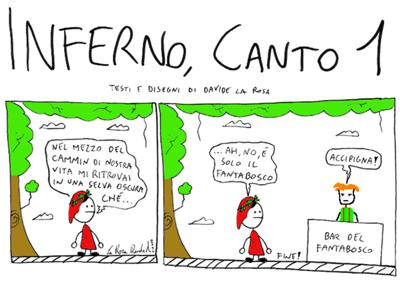
\includegraphics[scale=0.75]{inferno.jpeg}
\caption{Diagramma delle classi dettagliato che illustra i package
\nolinkurl{mytalk.client.iPresenter.iUser.iLogicUser} e mytalk.client.presenter.user.logicUser.}
\end{figure}
\end{center}

Il problema delle \index{immagini} immagini e' che sono difficili da impaginare quando \LaTeX \ f\`{a} i capricci :(
\\
testo a casaccio...\cite{webRTC}
\\
I have been wondering how to make a separate bibliography of my own publications as an appendix in my dissertation. Vincent pointed me to multibib and its siblings, and then I came across this FAQ about all the glories of multiple bibliographies. Doesn’t look like the easiest thing to get going, but I’ll dive into it and see if I manage to get out of it successfully.\cite{som}

%per importare da file:
%\input{sezione.tex}
%\newpage

%per ora non serve la biblio
%\bibliography{../bibliografia}
\newpage
\section{Capitolato C3 UMAP}
\paragraph{Descrizione}

Questo capitolato richiede l'implementazione di un sistema per la  raccolta e la elaborazione di dati eterogenei, dando inoltre la possibilità all'utente finale di leggere I dati e l'analisi fatta sugli stessi da un engine predittivo.
\paragraph{Requisiti obbligatori}  
\subparagraph{Sviluppo di :}	
	\begin{enumerate}
	\item Frontend
	\item Business Logic API 
	\item Engine predittivo
	\item Broker MQTT 
	\end{enumerate}

\paragraph{Aspetti Positivi:}
\begin{enumerate}
\item	Le tecnologie necessarie per svolgere il capitolato sono svariate (java, mongoDB, AWS , html e molte altre ) il che permetterebbe al gruppo di venire in contatto con strumenti nuovi ed estremamente utili in ambito lavorativo.
\end{enumerate}
\paragraph{Fattori di Rischio:}
	\begin{enumerate}
\item	Lo studio e l'apprendimento delle tecnologie necessarie sicuramente risulterebbe in uno sforzo notevole da parte di ogni componente del gruppo.

\item	Un altra difficolta risiede nella realizzazione del motore predittivo dato che al gruppo mancano totalmente le idee e le conoscenze per concepire l'elaborazione di dati eterogenei, considerando anche il fatto che durante la presentazione non sono	stati dati spunti a riguardo.
\item	Il sistema da realizzare sarebbe incredibilmente amplio.
\end{enumerate}
\newpage
\section{Capitolato C4 MaaS}
\paragraph{Descrizione}
Maas è basato su un prodotto di nome Maap, che è un database noSql per il trattamento di dati Business attraverso un interfaccia grafica permettendone l'utilizzo a persone che non sono esperte di database.Il committente richiede che questo prodotto diventi un servizio gestito attraverso un account web che dia la possibilità di eliminare l'onere all'utente di eseguire la preparazione e l'installazione di Maap.

\paragraph{Requisiti obbligatori}
\begin{enumerate}




\item	Le tecnologie richieste includono:

\begin{enumerate}



\item Node.js per il backend. MaaS deve essere in Long Term Support [LTS] versione Argon;

\item	MongoDB, versione maggiore di 3.x come database per l'applicazione; 

\end{enumerate}

\item Il Sistema deve essere costruito usando un framework di alto livello per Node.js. Noi fortemente consigliamo di usare IBM loopback.

\item Il sistema deve essere schierabile con Heroku.
 
\item	Il codice sorgente deve essere pubblicato e versionato   usando github oppure bitbucket. 
\end{enumerate}
\paragraph{Aspetti Positivi:}
\begin{enumerate}


\item	Potenzialmente la mole di lavoro e la complessità dello stesso potrebbero essere esigue dato che il capitolato si basa già su un prodotto esistente.

\item	Alcune delle tecnologie a supporto del capitolato potrebbero essere , anche se in modo parziale, già note al gruppo ( html, css, un servizio di	database, java ).
\end{enumerate}
\paragraph{Fattori di Rischio:}
	\begin{enumerate}
\item	L'argomento risulta essere poco stimolante, dato che la parte più interessante sarebbe stata la creazione di Maap che è già stato implementato.

\item	Essendo il committente una Startup con risorse di tempo, personale e	finanze limitate è possibile che sia difficile aiutare e seguire in	gruppo di lavoro in caso di problemi o dubbi inerenti al progetto.
\end{enumerate}

\end{document}
